%Lab Report
\documentclass[12pt,titlepage, a4paper]{article}
 \usepackage[german]{babel}
 \usepackage[utf8]{inputenc}
 \usepackage{graphicx}
 
\begin{document}

\title{Report\\LAB Kognitive Robotik}

\author{Münstermann,  Cedrick\\  Krombach, Nicola\\[1cm]
	Autonomous Intelligent Systems\\ \textsc{Universität Bonn}\\}



\maketitle


\section*{Abstract}


\section{Einleitung}

Im Rahmen der Projektgruppe Kognitive Robotik sollten in diesem Jahr die Aufgaben der European Robotics Challenges\footnote{http://www.euroc-project.eu/} bearbeitet werden. 
Die Aufgaben der European Robotics Challenges unterteilen sich dabei in drei Challenges, die wiederum verschiedene Unteraufgaben haben:

\begin{itemize}
 \item Challenge 1: Stationäre Manipulationsroboter in Kooperation mit Menschen (Track 1 \& 2)
 \item Challenge 2: Mobile Manipulationsroboter für die Logistik (Track 1 \& 2)
 \item Challenge 3: Flugroboter für industrielle Inspektion (Track 1 \& 2)
\end{itemize}

blabla mehr zu euroc? \\
Autonome Flugroboter eignen sich aufgrund ihres flexiblen Aufbaus und der Möglichkeit schwer zugängliche Objekte anzufliegen, besonders für die Inspektion und Überwachung von sehr großen industriellen
Anlagen oder Infrastrukturen. Dabei sollen sie autonom agieren, sodass auf die Abhängigkeit von einem Piloten verzichtet werden kann.
Auch für die Inspektion von gefährlichen Umgebungen eignet sich ein autonomer Flugroboter.

Unsere Gruppe befasste sich mit dem ersten Track der dritten Challenge, bei welchem die Lokalisierung des MAV und die 3D-Rekonstruktion der Umgebung mit Hilfe von Stereo-Bildern
im Vordergrund stand.



\section{Aufgabenstellung} 
In dem ersten Track von Challenge 3 geht es vorrangig um die Verarbeitung von visuellen Informationen, um die Pose des MAV zu schätzen und schließlich eine Karte von der Umgebung aufzubauen.



\subsection{Task 1 - Visuelle Lokalisierung}
In der ersten Aufgabe ging es darum aus Stereobildern eine 6D-Pose zu schätzen. Dazu wurden realistische Datensätze mit unterschiedlichen Schwierigkeiten zur Verfügung gestellt.
Ausschließlich anhand von diesen Datensätzen sollte nun die Lokalisierung erfolgen. Für die Evaluation war sowohl die lokale Genauigkeit als auch die Echtzeitfähigkeit der Berechnung entscheidend.
Eine \"Ubersicht der Evaluierungskriterien und Punktevergabe findet sich in \cite{blaURL}.

Vision based localization\\
Localize w.r.t. starting point\\
Local accuracy/consistency\\
Real-time computation!\\

\begin{figure}
 \centering
 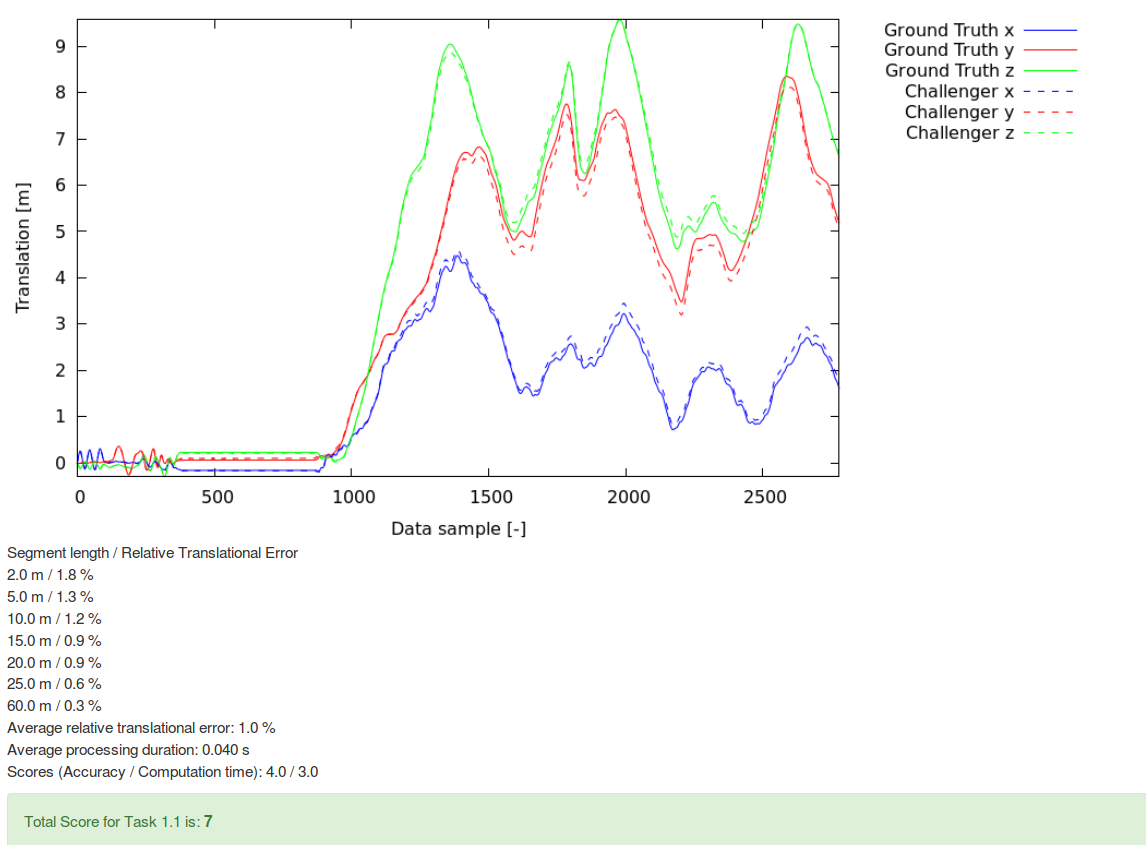
\includegraphics[width=\textwidth]{./Screens/t1_opt2_april.png}
 % t1_opt2_april.png: 1243x912 pixel, 96dpi, 32.88x24.13 cm, bb=0 0 932 684
\end{figure}


				
\subsection{Task 2 - 3D-Rekonstruktion}

Reconstruct environment in order to create a 3-D occupancy grid
Camera poses are given
create occupancy grid from depth images
Real-time computation, but over the whole dataset



\section{Experimente}




\section{Zusammenfassung}


\end{document}
